\chapter{Bounds from \texorpdfstring{$\pi^+$}{pion} decay spectrum}
\label{ch:BoundsPI}
As was seen in the previous section, pions decay almost exclusively in a muon and the corresponding neutrino. The clean background and theoretically well understood decay mode establish it as a useful scenario to investigate BSM models that influence the decay. For this work the most important feature are the two final state leptons. 
The simplicity of the production and identification of pions in collider experiments provide a rich experimental data source. 
One data set that can be used to constrain leptophilic mediator models is found in \emph{Improved Search for Heavy Neutrinos in the Decay $\pi\rightarrow e\nu$} \cite{Aguilar-Arevalo:2017vlf} by the PIENU Collaboration. 
The aim of this collaboration was to measure the  branching ration $R_{e/\mu}^\pi$ and thus test lepton universality more precise than ever before. 
The experiment used TRIUMFs M13 beam of pions that were creates by a proton beam hitting a Beryllium target. The fragments were then selected and collimated to form the pion beam consisting of 84\% $\pi^+$, 14\%$\mu^+$ and 2\%$e^+$. 
Pions were then distinguished from the other constituents by their energy loss in scintillators and subsequently stopped in the detector. These then decayed at rest. 
The resulting positron energy spectrum contains besides the pure $\pi^+\rightarrow e^+\nu_e$ decays also positrons from the decay chain $\pi^+\rightarrow \mu^++\nu_\mu \rightarrow e^+ \nu_e +\nu_\mu$ that are distinguished by fitting to Monte Carlo simulations or their timing and direction. 
The total spectrum and its constituents are shown in figure \ref{fg:PiENuSpectrum}.
\begin{figure}[H]
  \centering
    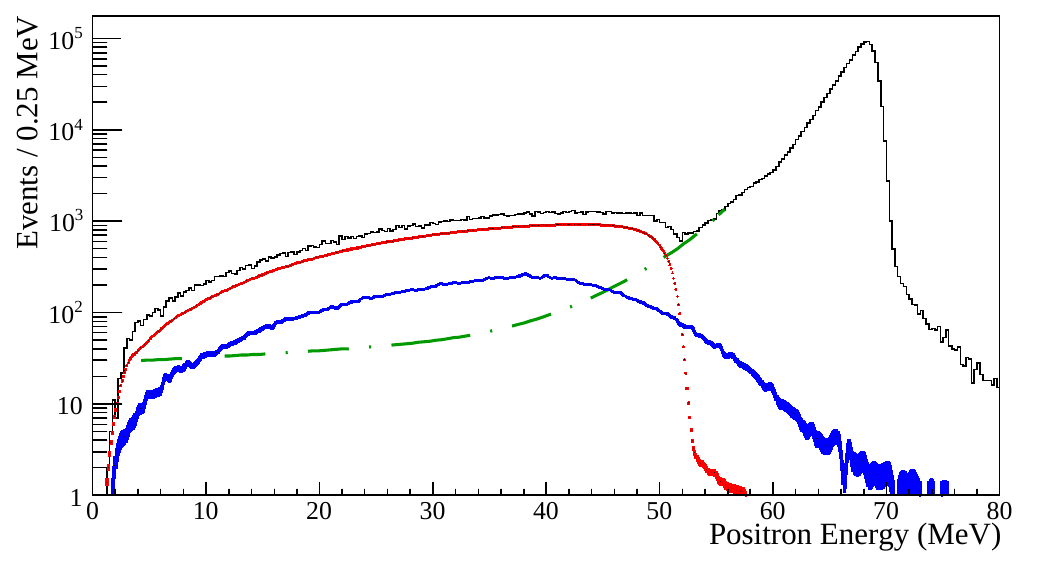
\includegraphics[width=0.8\textwidth]{imgs/graph}
    \caption{Backgound suppressed positron spectrum (black), with components from muon decays in flight (blue), $\pi^+\rightarrow e^+\nu_e$ (green) and $\pi^+\rightarrow \mu^++\nu_\mu \rightarrow e^+ \nu_e +\nu_\mu$ (red)
    taken from \cite{Aguilar-Arevalo:2017vlf}}
    \label{fg:PiENuSpectrum}
\end{figure}
The difference between the data and the fit can then be used to look for signs of new physics. This was then used to look for extra peaks is the spectrum that would indicate heavy neutrinos. The absence of any additional structure was used to constrain the neutrino mixing matrix elements in the mass region $60-135$MeV at 90\% C.L.

The same data set can conveniently be used to search for other sources of new physics. Most important in this work the diagram shown in figure \ref{fg:PiENuBSMGraphsScalar} can be used to extract constraints on the electron-scalar mediator coupling,
\begin{figure}[H]
\centering
\scalebox{1}{%
\begin{tikzpicture}
\begin{feynman}
\vertex (a) {\(\pi^{+}\)};
\vertex [right=of a] (b);
\vertex [right=of b] (c);
\vertex [above right=of c] (f1){\(\nu_e\)};
\vertex [below right=of c] (d);
\vertex [above right=of d] (f2){\(\phi\)};
\vertex [below right=of d] (f3){\(e^+\)};
\diagram* {
(a) -- [scalar] (b) -- [boson, edge label'=\(W^{+}\)] (c),
(c) -- [fermion] (f1),
(c) -- [anti fermion] (d),
(d) -- [anti fermion] (f3),
(d) -- [scalar] (f2)
};
\end{feynman}
\end{tikzpicture}
}

\caption{Pion-decay contribution with a scalar mediator}
\label{fg:PiENuBSMGraphsScalar}
\end{figure}
while the diagrams shown in figure \ref{fg:PiENuBSMGraphsVector} can be used to constrain the dark photon model where the vector couples to the electron. 
\begin{figure}[h]
\centering
\begin{subfigure}{.5\textwidth}
\centering
  \begin{tikzpicture}
\begin{feynman}
\vertex (a) {\(\pi^{+}\)};
\vertex [right=of a] (b);
\vertex [right=of b] (c);
\vertex [above right=of c] (f1){\(\nu_e\)};
\vertex [below right=of c] (d);
\vertex [above right=of d] (f2){\(A'\)};
\vertex [below right=of d] (f3){\(e^+\)};
\diagram* {
(a) -- [scalar] (b) -- [boson, edge label'=\(W^{+}\)] (c),
(c) -- [fermion] (f1),
(c) -- [anti fermion] (d),
(d) -- [anti fermion] (f3),
(d) -- [boson] (f2)
};
\end{feynman}
\end{tikzpicture}
\end{subfigure}%
\begin{subfigure}{.5\textwidth}
\centering
\begin{tikzpicture}
\begin{feynman}
\vertex (a) {\(\pi^{+}\)};
\vertex [right=of a] (b);
\vertex [right=of b] (c);
\vertex [above right=of c] (d);
\vertex [above right=of d] (f1){\(\nu_e\)};
\vertex [below right=of d] (f2){\(A'\)};
\vertex [below right=of c] (f3){\(e^+\)};
\diagram* {
(a) -- [scalar] (b) -- [boson, edge label'=\(W^{+}\)] (c),
(c) -- [fermion] (d)--[fermion](f1),
(c) -- [anti fermion] (f3),
(d) -- [boson] (f2)
};
\end{feynman}
\end{tikzpicture}

\end{subfigure}
\caption{Pion-decay contribution with a spin 1 mediator}
\label{fg:PiENuBSMGraphsVector}
\end{figure}
To this end, seven benchmark masses $1\cdot10^{-4}$GeV, $5\cdot10^{-4}$GeV, $1\cdot10^{-3}$GeV, $5\cdot10^{-3}$GeV, $1\cdot10^{-2}$GeV, $5\cdot10^{-3}$GeV and $1\cdot10^{-1}$GeV were chosen.
For each scenario a set of 10.000 Monte Carlo events for the new physics processes were generated. 
These were then put in a histogram that had the same binning as the dataset from the heavy neutrino search. 
\begin{equation}
\chi^2\equiv \sum^\nu_{i=1}\frac{(x_i-\mu_i)^2}{\sigma_i^2}
\end{equation}
The total number of particles in this histogram is then varied and was then subjected to a $\chi^2$ test to establish a 95\% C.L. bound on the  relative abundance of the processes in this spectrum $\alpha$. This is shown in figure \ref{fg:PionExamplePlots} for a 100MeV dark photon.
\begin{figure}[h]
  \centering
    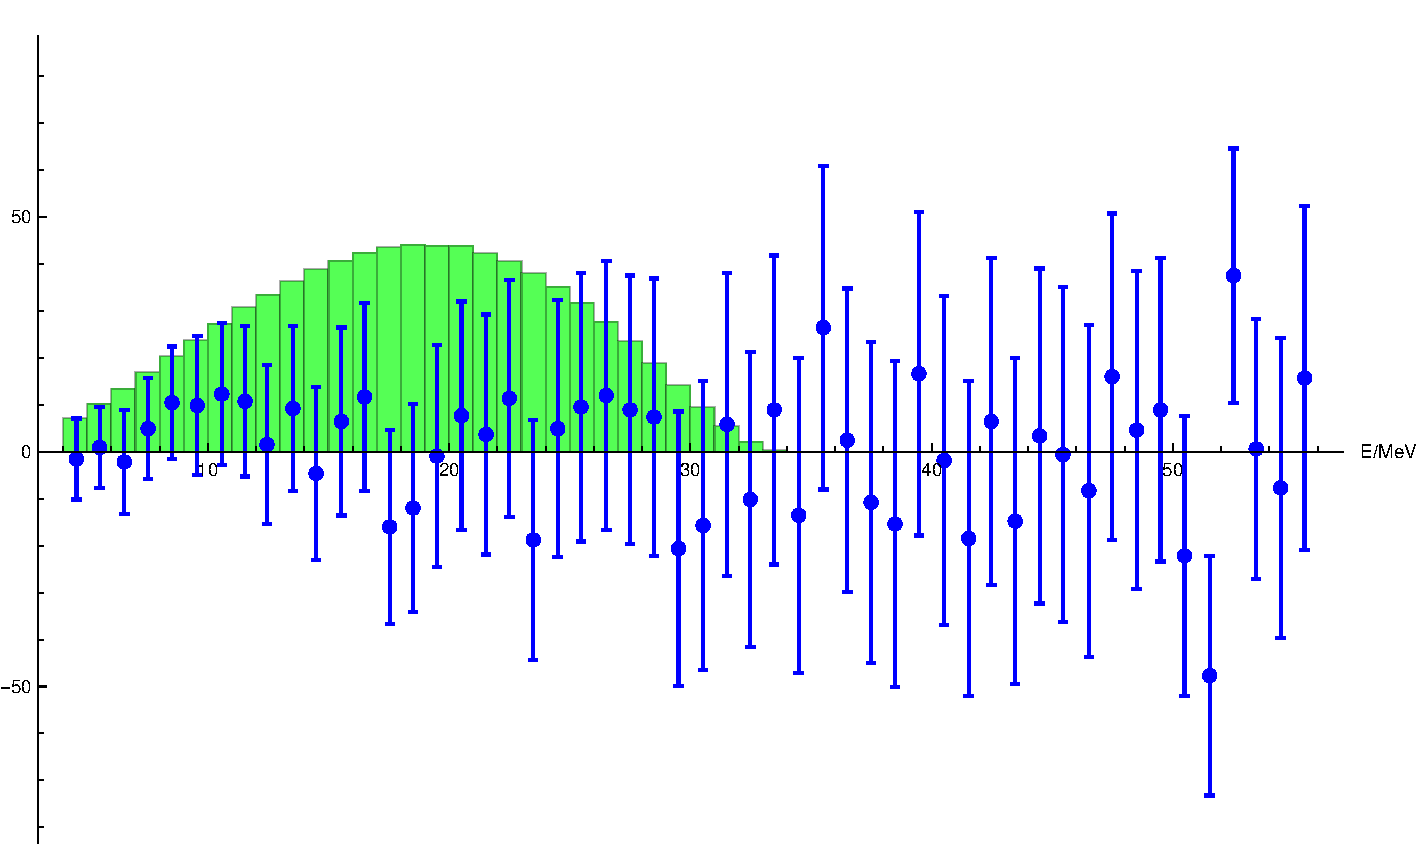
\includegraphics[width=0.6\textwidth]{imgs/PionExamplePlot}
    \caption{Datapoints from \cite{Aguilar-Arevalo:2017vlf}(blue) and positron energy spectrum for a 100MeV vector scaled such that the coupling saturates the 90\% C.L. bound} 
    \label{fg:PionExamplePlots}
\end{figure}
\begin{equation}
\alpha \gtrsim \frac{\Gamma(\pi^+\rightarrow e^+ \nu_e + \phi/A')}{\Gamma(\pi^+\rightarrow e^+ \nu_e)}
\end{equation}
This is then used to extract the coupling constants 
\begin{equation}
e_l'^2\lesssim \frac{\alpha\Gamma(\pi^+\rightarrow e^+ \nu_e)}{\Gamma(\pi^+\rightarrow e^+ \nu_e + \phi/A')|_{e_l'=1}}.
\end{equation}

\section{Results}
\begin{figure}[H]
  \centering
    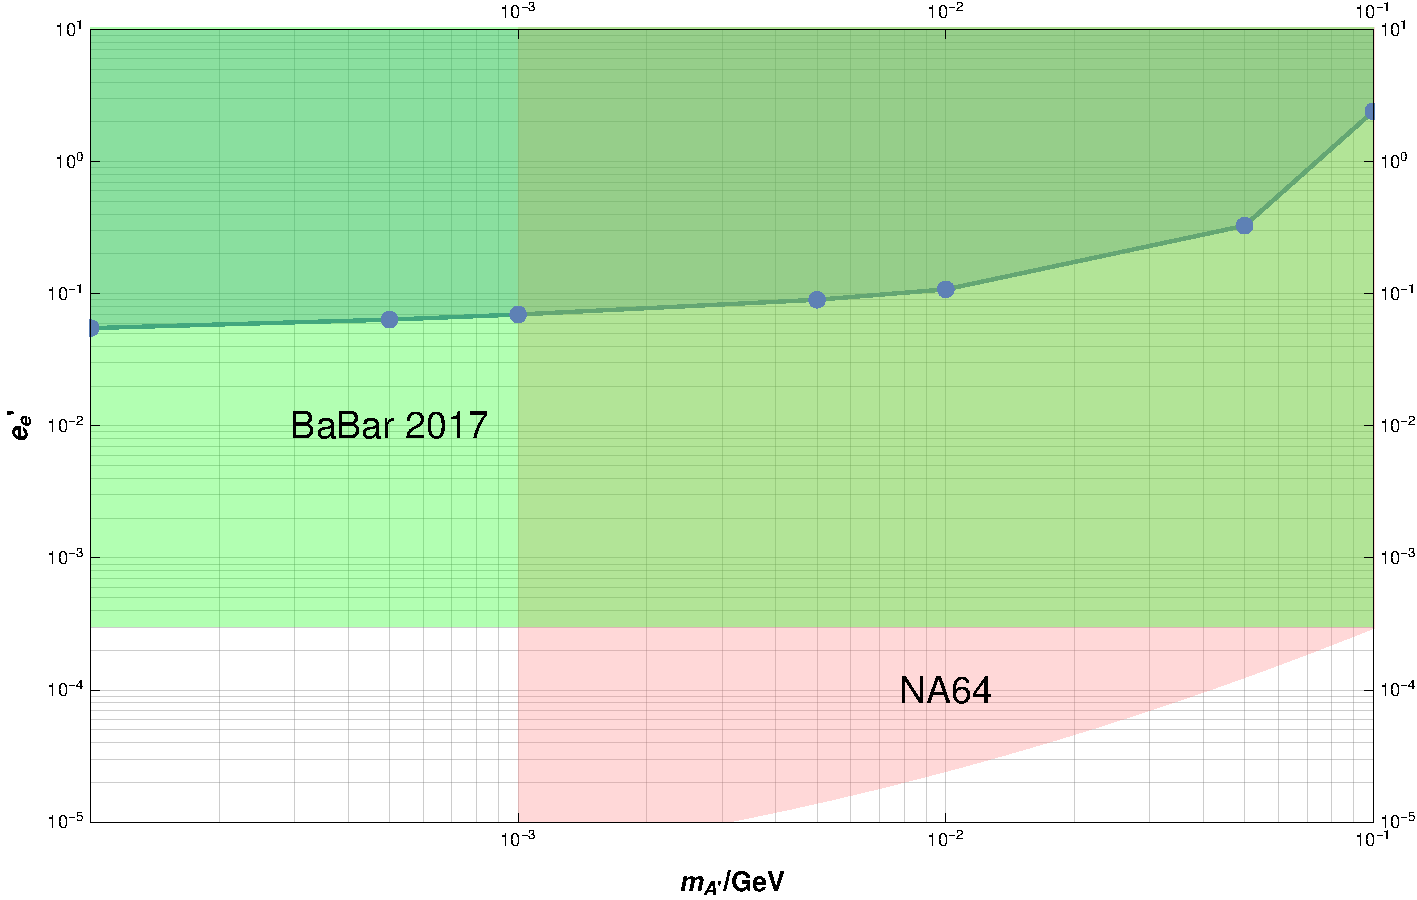
\includegraphics[width=0.8\textwidth]{imgs/PionSpectrumVector}
    \caption{95\% C.L. bounds on the vector couplings to the electron (blue)}
    \label{fg:PiSpectrumVectorBounds}
\end{figure}

\begin{figure}[H]
  \centering
    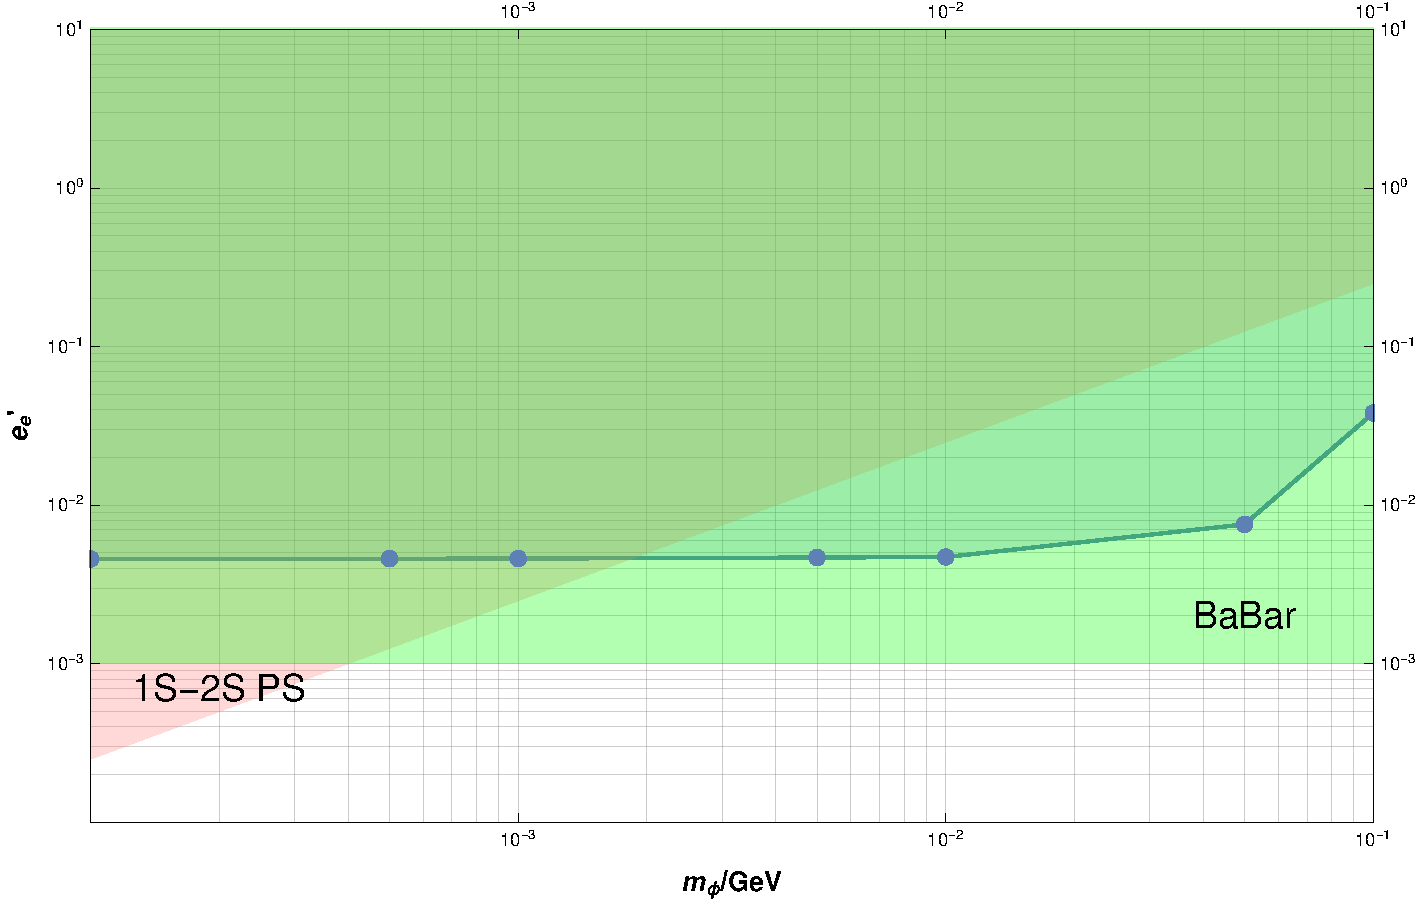
\includegraphics[width=0.8\textwidth]{imgs/PionSpectrumScalar}
    \caption{95\% C.L. bounds on the scalar couplings to the electron (blue) with bounds from 1S-2S transitions in positronium (red, 95\% C.L.) and BABAR (green, 95\% C.L.)}
    \label{fg:PiSpectrumScalarBounds}
\end{figure}

The extracted relative abundance $\alpha$ between the two models is of a similar order, despite the drastically different bounds on the couplings.  
\section{Discussion}
The bounds on the vector interaction with the electron is far from being competitive. Even strong experimental improvements will not lead to new bounds beyond the BABAR constraints.
On the other hand the bounds for the scalar interaction are much stronger, despite similar values of $\alpha$ compares to the vector case. The reason is that the scalar removes the chiral suppression whereas it stays in tact for the vector interaction. This leads to drastically larger decay width which in turn requires smaller coupling constants to be unobserved. Nevertheless this also doesn't lead to better bounds than the ones currently available. In this case a realistic improvement of experimental data could lead to better bounds than from BABAR for $m_\phi>\SI{300}{\kilo\eV}$.